% arara: lualatex
\pdfoptionpdfminorversion 7
\documentclass{beamer}
\AtBeginSection{\frame{\sectionpage}}

\defbeamertemplate{section page}{mine}[1][]{%
  \begin{centering}
    {\usebeamerfont{section name}\usebeamercolor[fg]{section name}#1}
    \vskip1em\par
    \begin{beamercolorbox}[sep=12pt,center]{part title}
      \usebeamerfont{section title}\insertsection\par
    \end{beamercolorbox}
  \end{centering}
}
\setbeamertemplate{section page}[mine]

\usepackage{pgfplots}

\title{High Pressure Ignition Chemistry of Alternative Fuels}
\author{Bryan W. Weber}
\institute{Prepared for Ph.D. Defense}
\date{June 19, 2014}

\beamertemplatenavigationsymbolsempty

\setbeamertemplate{footline}
{%
\begin{beamercolorbox}[sep=2mm]{}

\includegraphics[height=0.25in]{logo}
\hfill
{\color{gray} \insertpagenumber{}/\insertpresentationendpage}
\end{beamercolorbox}
}%

\graphicspath{ {figures/} }

\begin{document}

\maketitle

\begin{frame}{We use a lot of fuels to power the world}
    \only<1,3>{
        \begin{center}
            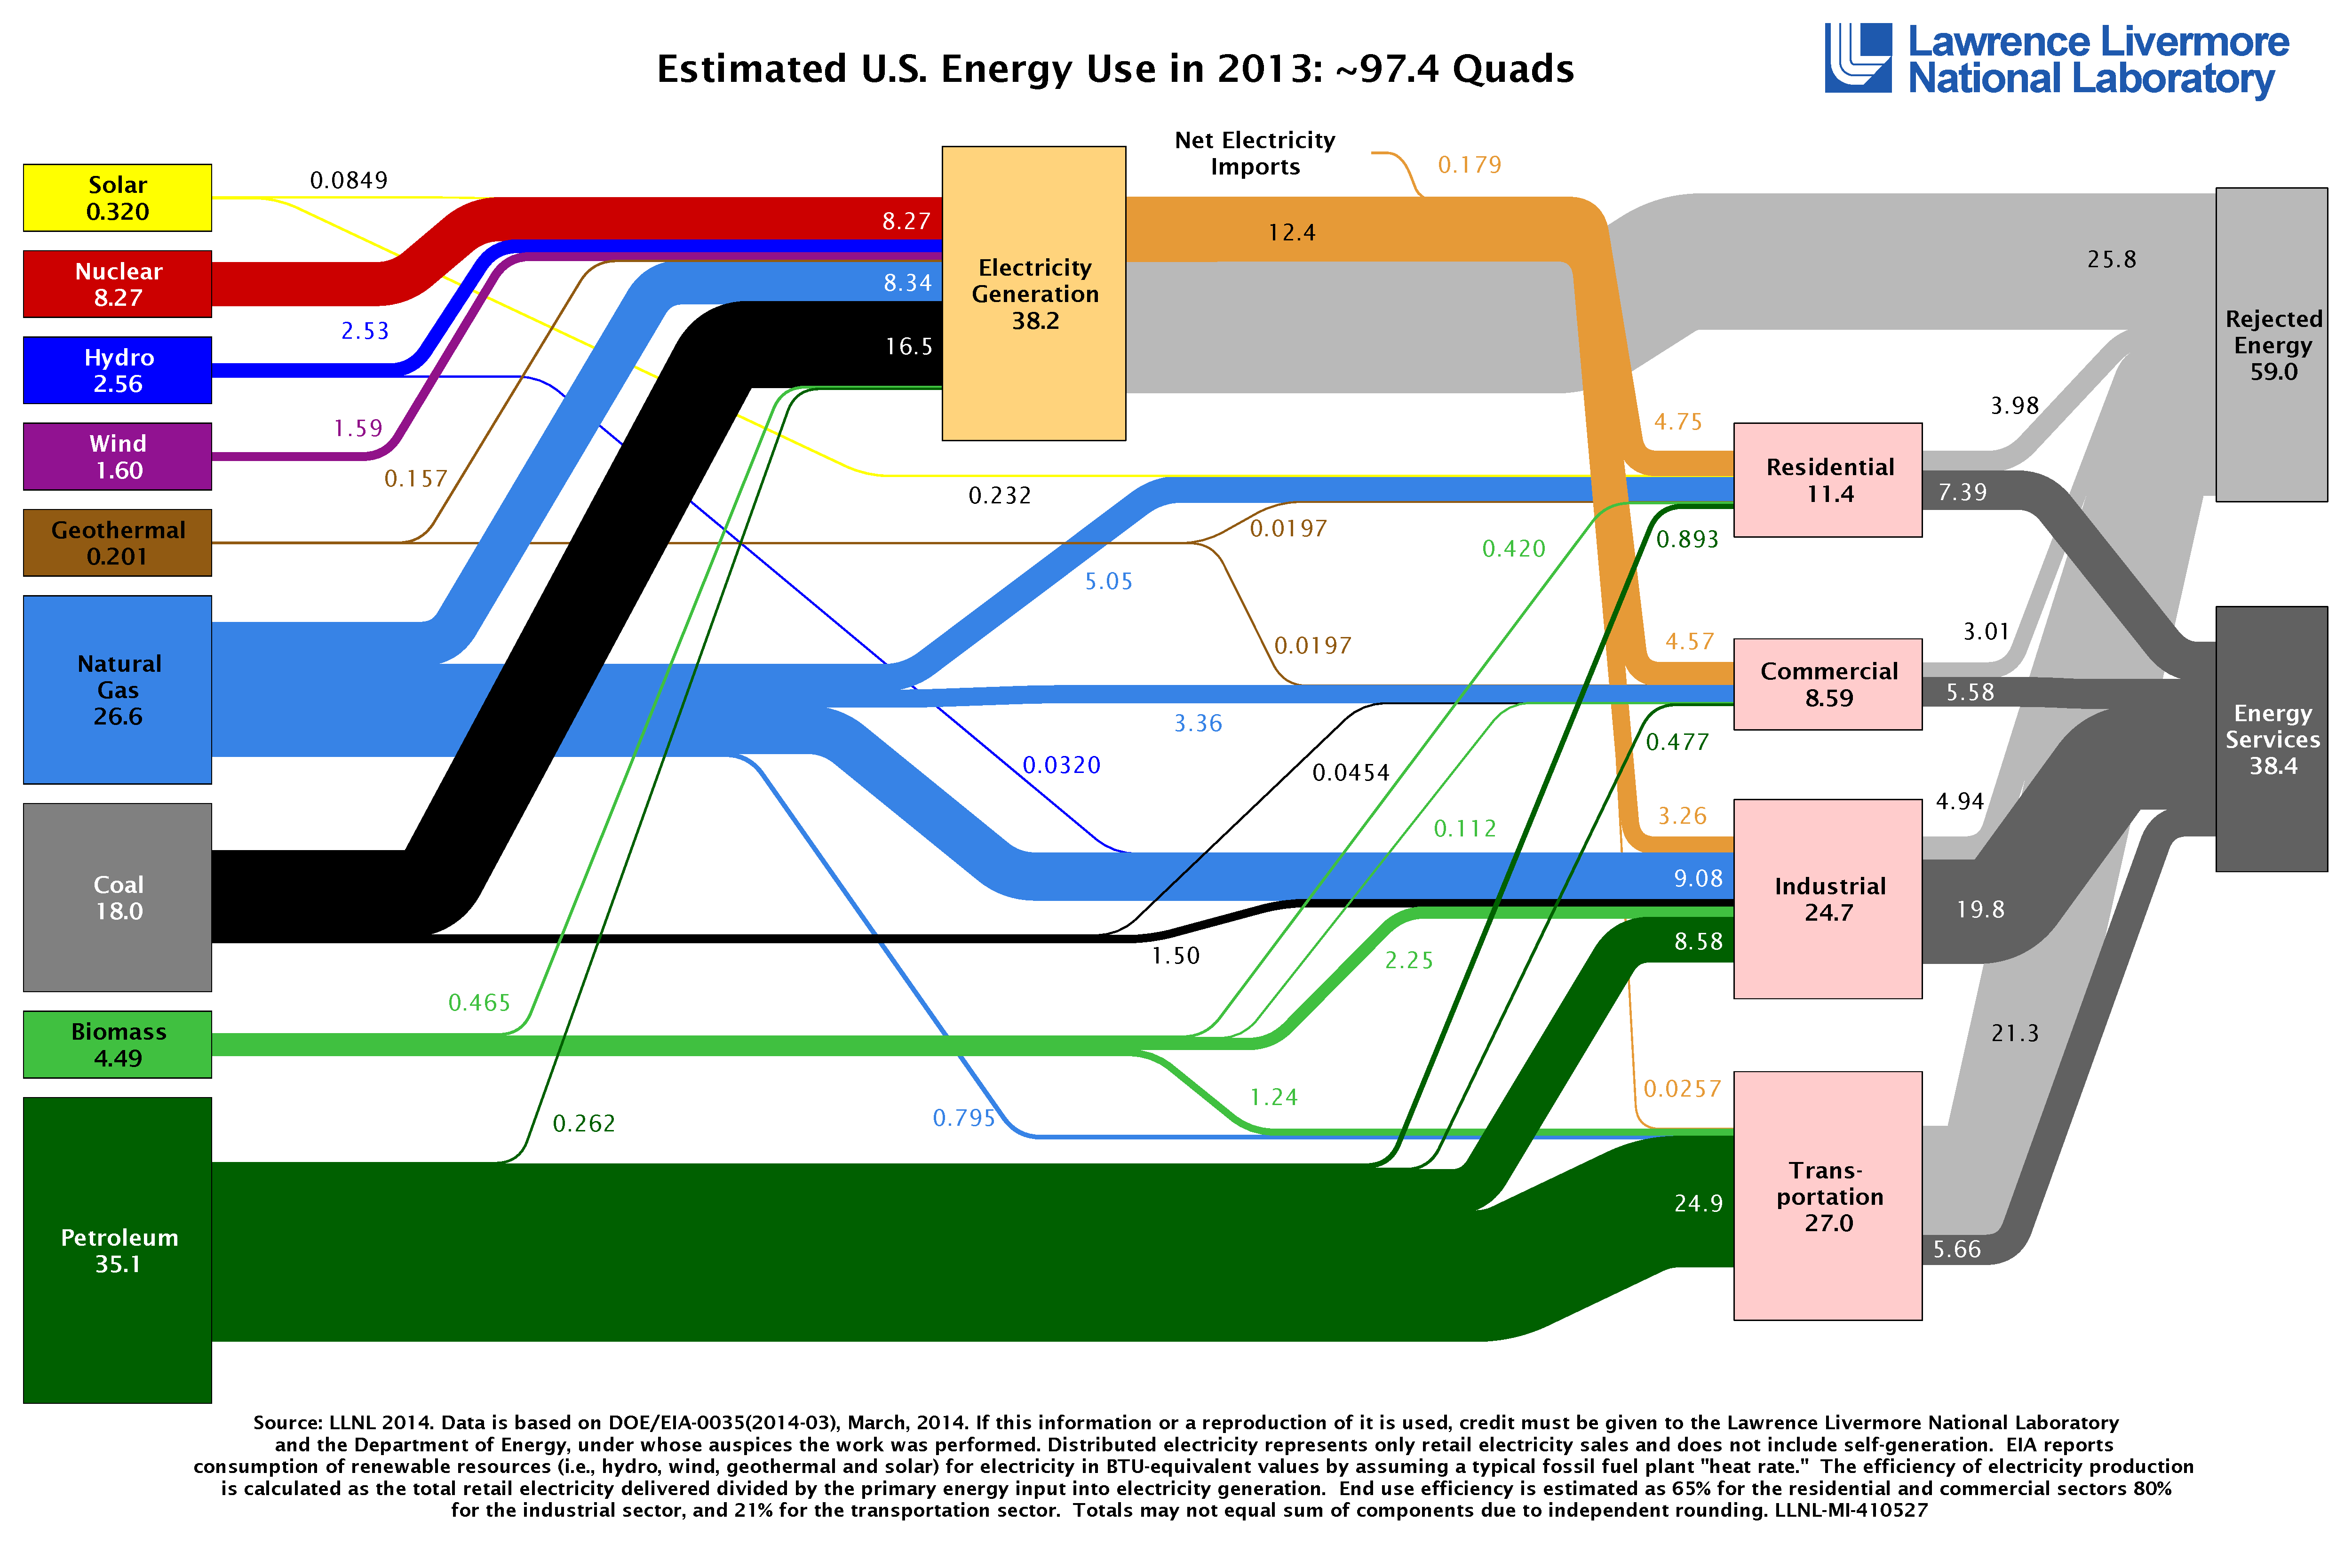
\includegraphics[width=\textwidth]{2013USEnergy}
        \end{center}
    }
    \only<2>{Could drive to the moon and back over 180 million times in a Tesla Model S with the amount of energy we use annually}
    % \begin{center}
        % \includegraphics[width=\textwidth]{me-to-moon}
    % \end{center}
    \only<4>{
        \begin{itemize}
            \item Combustion is predicted to remain the dominant energy conversion process for many years into the future
            \item The combustion of fossil fuels has been implicated in a number of harmful effects on human health, the environment, and the economy
            \item Two solutions have been proposed:
                \begin{itemize}
                    \item Better engines
                    \item Better fuels
                \end{itemize}
        \end{itemize}
    }
\end{frame}

\begin{frame}{Better engines have higher efficiency and lower emissions}
John Dec image
\end{frame}

\begin{frame}{Better fuels reduce emissions and eliminate dependence on fossil fuels}
    \begin{center}
        % 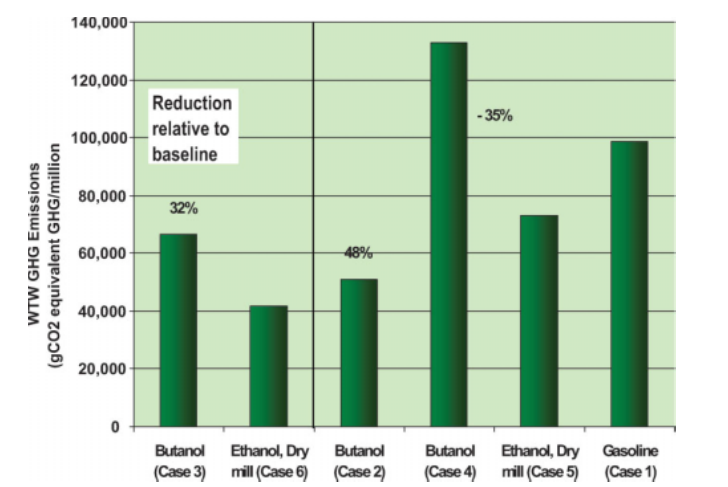
\includegraphics[width=\textwidth,height=0.85\textheight,keepaspectratio]{butanol-benefits}
        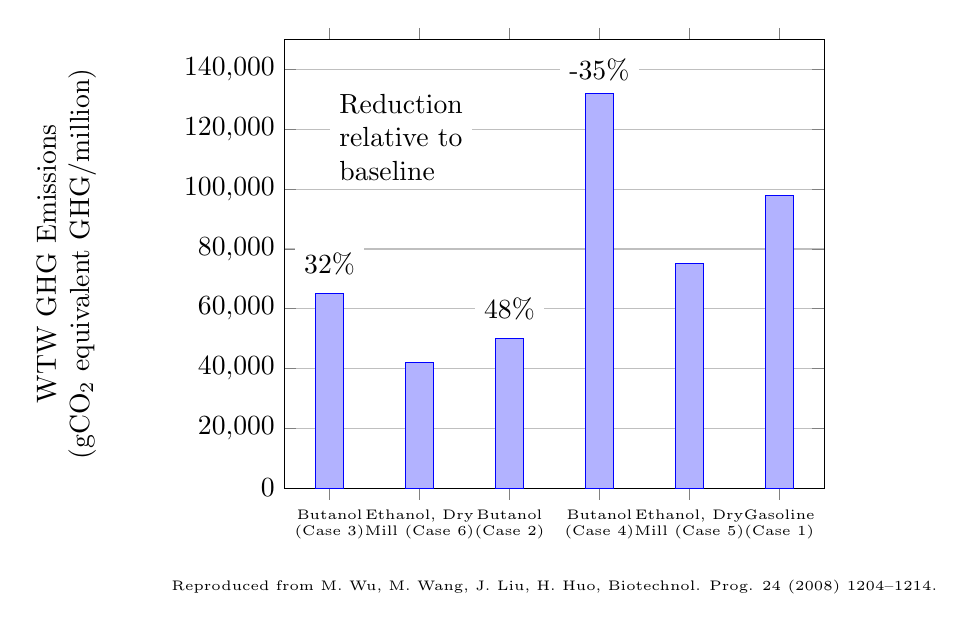
\begin{tikzpicture}
        \begin{axis}[
            ybar,
            scaled y ticks=false,
            ymin=0,ymax=150000,
            ytick={0,20000,40000,60000,80000,100000,120000,140000},
            yticklabel style={/pgf/number format/fixed},
            xtick={1,2,3,4,5,6},
            xticklabels={{Butanol\\(Case 3)}, {Ethanol, Dry\\Mill (Case 6)}, {Butanol\\(Case 2)}, {Butanol\\(Case 4)}, {Ethanol, Dry\\Mill (Case 5)}, {Gasoline\\(Case 1)}},
            xticklabel style={align=center,font=\tiny},
            ymajorgrids,
            ylabel={WTW GHG Emissions\\(gCO$_2$ equivalent GHG/million)},
            ylabel style={align=center,yshift=25pt},
            xlabel={Reproduced from M. Wu, M. Wang, J. Liu, H. Huo, Biotechnol. Prog. 24 (2008) 1204--1214.},
            xlabel style={font=\tiny,yshift=-8pt},
        ]
        \addplot coordinates {(1,65000) (2,42000) (3,50000) (4,132000) (5,75000) (6,98000)};
        \node[fill=white] at (axis cs:1,75000) {32\%};
        \node[fill=white] at (axis cs:3,60000) {48\%};
        \node[fill=white] at (axis cs:4,140000) {-35\%};
        \node[fill=white, anchor=north west, align=left] at (axis cs:1,135000) {Reduction\\relative to\\baseline};
        \end{axis}
        \end{tikzpicture}
    \end{center}
\end{frame}

\begin{frame}
    \begin{center}
        {\Large What kind of research can we do to push these solutions along?}
    \end{center}
\end{frame}

\begin{frame}{We can do biological research to produce the fuels}
    \begin{center}
        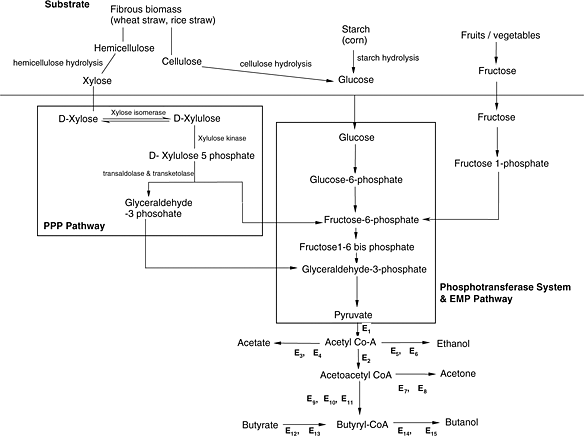
\includegraphics[width=\textwidth]{butanol-production}
    \end{center}
    \begin{textblock*}{50mm}(5mm,65mm)
        {\tiny Reproduced from A. Ranjan and V. S. Moholkar, Int. J. Energy Res., 36 (2012) 277--323}
    \end{textblock*}
\end{frame}

\begin{frame}{We can do engineering research on how the fuels will behave}
    \begin{itemize}
        \item We need to know the physical properties
        \begin{itemize}
            \item Density
            \item Viscosity
            \item \ldots
        \end{itemize}
        \item We need to know the \alert<2->{combustion properties}
        \begin{itemize}
            \item Heat of combustion
            \item Propensity to generate pollutants
            \item Reactivity
            \item \ldots
        \end{itemize}
    \end{itemize}
\end{frame}

\begin{frame}{What tools does combustion research use?}
    \vspace{0.5cm}
    \only<3->{\setbeamercovered{transparent=15}}
    \begin{columns}
        \uncover<1,2>{
        \column{0.5\textwidth}
            Phenomenological Studies
            \begin{itemize}
                \item Engine Studies
                \item Octane Number
                \item \ldots
            \end{itemize}
        }
        \column{0.5\textwidth}<2->
            Fundamental Studies
            \begin{itemize}
                \item Ignition Delay
                \item Product Speciation
                \item \ldots
            \end{itemize}
    \end{columns}
    \vspace{0.5cm}
    \hspace{6.25cm} \tikzmark{right}
    \begin{itemize}
        \item<3-> Experiments \tikzmark{2nd}
        \begin{itemize}[<4- | invisible@-3>]
            \item Engine experiments
            \item \alert<7>{Homogeneous experiments}
            \item Heterogeneous experiments
        \end{itemize}
        \item<3->Modeling
        \begin{itemize}[<5- | invisible@-4>]
            \item Quantum chemical modeling
            \item \alert<7>{Reaction mechanisms}
            \item Computational fluid dynamics
                \tikzmark{4th}
        \end{itemize}
    \end{itemize}
    \begin{tikzpicture}[overlay, remember picture]
        \draw<6>[decoration={brace,amplitude=0.5em},decorate,ultra thick,red]
 ($(right)!(2nd.north)!($(right)-(0,1)$)$) --  ($(right)!(4th.south)!($(right)-(0,1)$)$);
        \path<6> ($(right)!(2nd.north)!($(right)-(0,1)$)$) --  ($(right)!(4th.south)!($(right)-(0,1)$)$) node[midway,align=left,anchor=west,red,xshift=0.25cm] {These efforts\\are complementary!};
    \end{tikzpicture}
\end{frame}

\begin{frame}{What phenomena am I trying to understand?}
    \begin{center}
        \only<+>{{\Large How do alternative fuels react at engine-relevant conditions?}}
        \only<+>{
            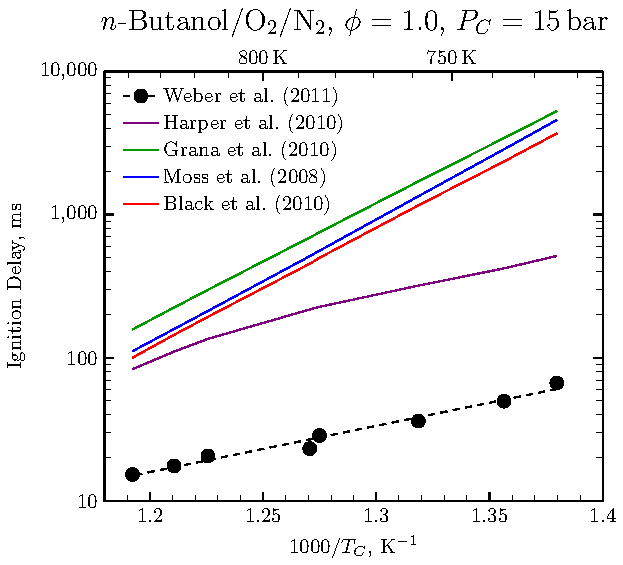
\includegraphics[height=0.8\textheight]{nbuoh-2010/nbuoh-2010}\\
            Until 2011, no one was aware that low-temperature chemistry would
            be important for alcohol fuels!
        }
    \end{center}
\end{frame}

\begin{frame}{What is low-temperature chemistry?}
    \begin{center}
    \begin{tikzpicture}
    \begin{semilogyaxis}[
        table/col sep=comma,
        ylabel style={align=center,yshift=-15pt},
        xlabel style={align=center,yshift=15pt},
        ylabel={Reactivity\\$\leftarrow$Higher\qquad\qquad Lower$\rightarrow$},
        xlabel={$\leftarrow$Higher\qquad\qquad Lower$\rightarrow$\\Temperature},
        yticklabels={,,},
        xticklabels={,,},
        xmin=0.7,xmax=1.5,
        ymin=0.02,ymax=200,
        tick style = {color=black, semithick},
        minor tick style={thin},
        axis line style={semithick},
        every axis plot/.append style={%
            semithick,
        },
        every axis legend/.append style={legend pos=south east,anchor=south east,font=\tiny},
        legend columns=1,
    ]
    \only<1->{\addplot[mark=*,blue,only marks,restrict x to domain=0.7:1.15] table[x=Alcohol-Tc, y=Alcohol-Ign] {figures/alcohol-models/model-data.csv};
    \addlegendentry{High Temperature Alcohol}}
    \only<2-6>{\addplot[only marks,mark=square*,red] table[x=Hi-T-Real-Tc, y=Hi-T-Real-Ign] {figures/alcohol-models/model-data.csv};
    \addlegendentry{High Temperature Alkane}}
    \only<3-6>{\addplot[no markers,cyan] table[x=Hi-T-Alc-Tc, y expr=\thisrow{Hi-T-Alc-Mod}*0.75] {figures/alcohol-models/model-data.csv};
    \addlegendentry{High Temperature Model}}
    \only<4->{\addplot[only marks,mark=oplus*,violet,restrict x to domain=1.15:1.5] table[x=Alcohol-Tc, y=Alcohol-Ign] {figures/alcohol-models/model-data.csv};
    \addlegendentry{Low Temperature Alcohol}}
    \only<5-6>{\addplot[only marks,mark=diamond*,black] table[x=Lo-T-Real-Tc, y=Lo-T-Real-Ign] {figures/alcohol-models/model-data.csv};
    \addlegendentry{Low Temperature Alkane}}
    \only<6>{\addplot[no markers,orange] table[x=Real-Mod-Tc, y=Real-Mod-Ign] {figures/alcohol-models/model-data.csv};
    \addlegendentry{Comprehensive Alkane Model}}
    \only<7->{\addplot[no markers,domain=0.8:1.4,gray] {1.4097*x^12.714};
    \addlegendentry{Comprehensive Alcohol Model}}
    \end{semilogyaxis}
    \end{tikzpicture}
    \end{center}
\end{frame}

\begin{frame}{What phenomena am I trying to understand?}
    \begin{center}
        \only<1>{
            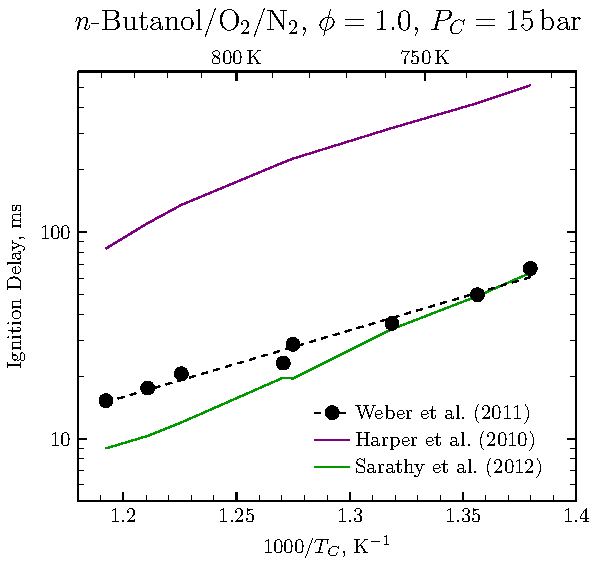
\includegraphics[height=0.8\textheight]{nbuoh-2014/nbuoh-2014}\\
            With low-temperature reaction classes added, models can
            better predict the ignition delay.
        }
    \end{center}
    \only<2>{
        \begin{columns}
            \column{0.45\textwidth}
                \centering
                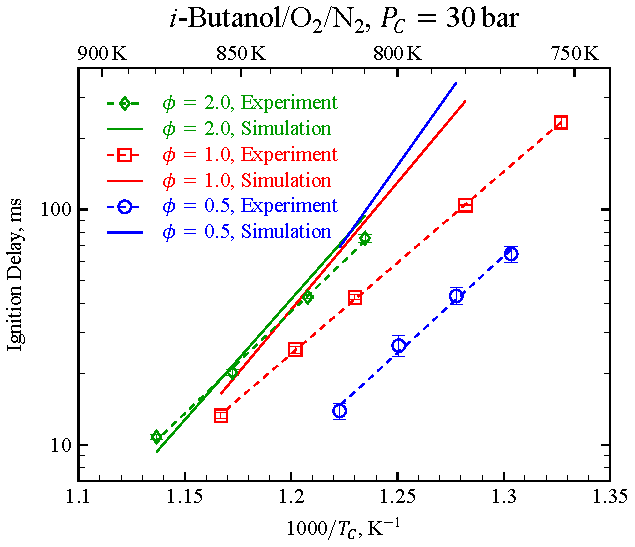
\includegraphics[width=\textwidth]{ibuoh-30o2sim}\\
                Weber et al. 8th US National Combustion Meeting 2013
            \column{0.45\textwidth}
                \centering
                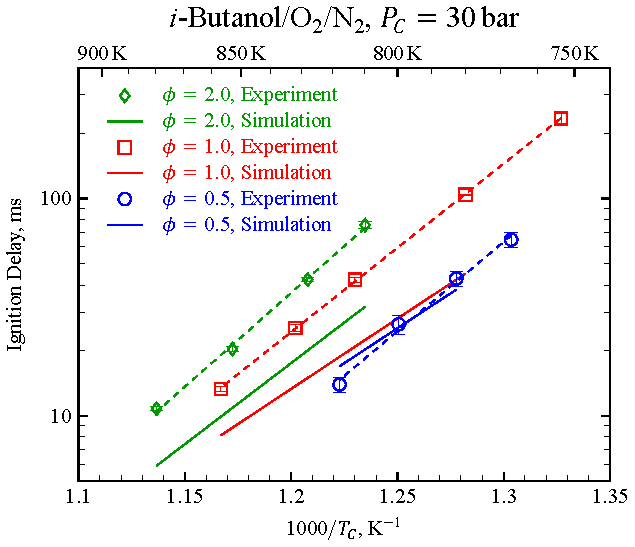
\includegraphics[width=\textwidth]{ibuoh-30o2sim-sar}\\
                Sarathy et al. Combust. Flame 2012
        \end{columns}
        \vspace{0.5cm}
        \begin{center}
            There is still some critical information missing from our
            understanding of high-pressure, low-temperature ignition
            of alternative fuels
        \end{center}
    }
\end{frame}

\section{Experimental Apparatuses}

\begin{frame}{Rapid Compression Machine}

    \begin{center}
        \includegraphics<+>[width=\textwidth]{rcm-photo}
        \includegraphics<+>[height=0.95\textheight]{ign-delay-def}
    \end{center}
\end{frame}

\begin{frame}{Rapid Sampling Apparatus}
    \only<-3>{
        \begin{columns}
            \column{0.4\textwidth}
                \begin{itemize}[<+->]
                    \item Sampling apparatuses have been used since the 1920's to study combustion chemistry
                    \item In the 1960's, the first sampling apparatus was adapted for an RCM
                    \item Sampling devices rapidly quench ongoing reactions so that species are determined at a discrete point in time
                \end{itemize}
            \column{0.6\textwidth}
                \centering
                \begin{minipage}[c][0.95\textheight][c]{\textwidth}
                \only<1>{
                    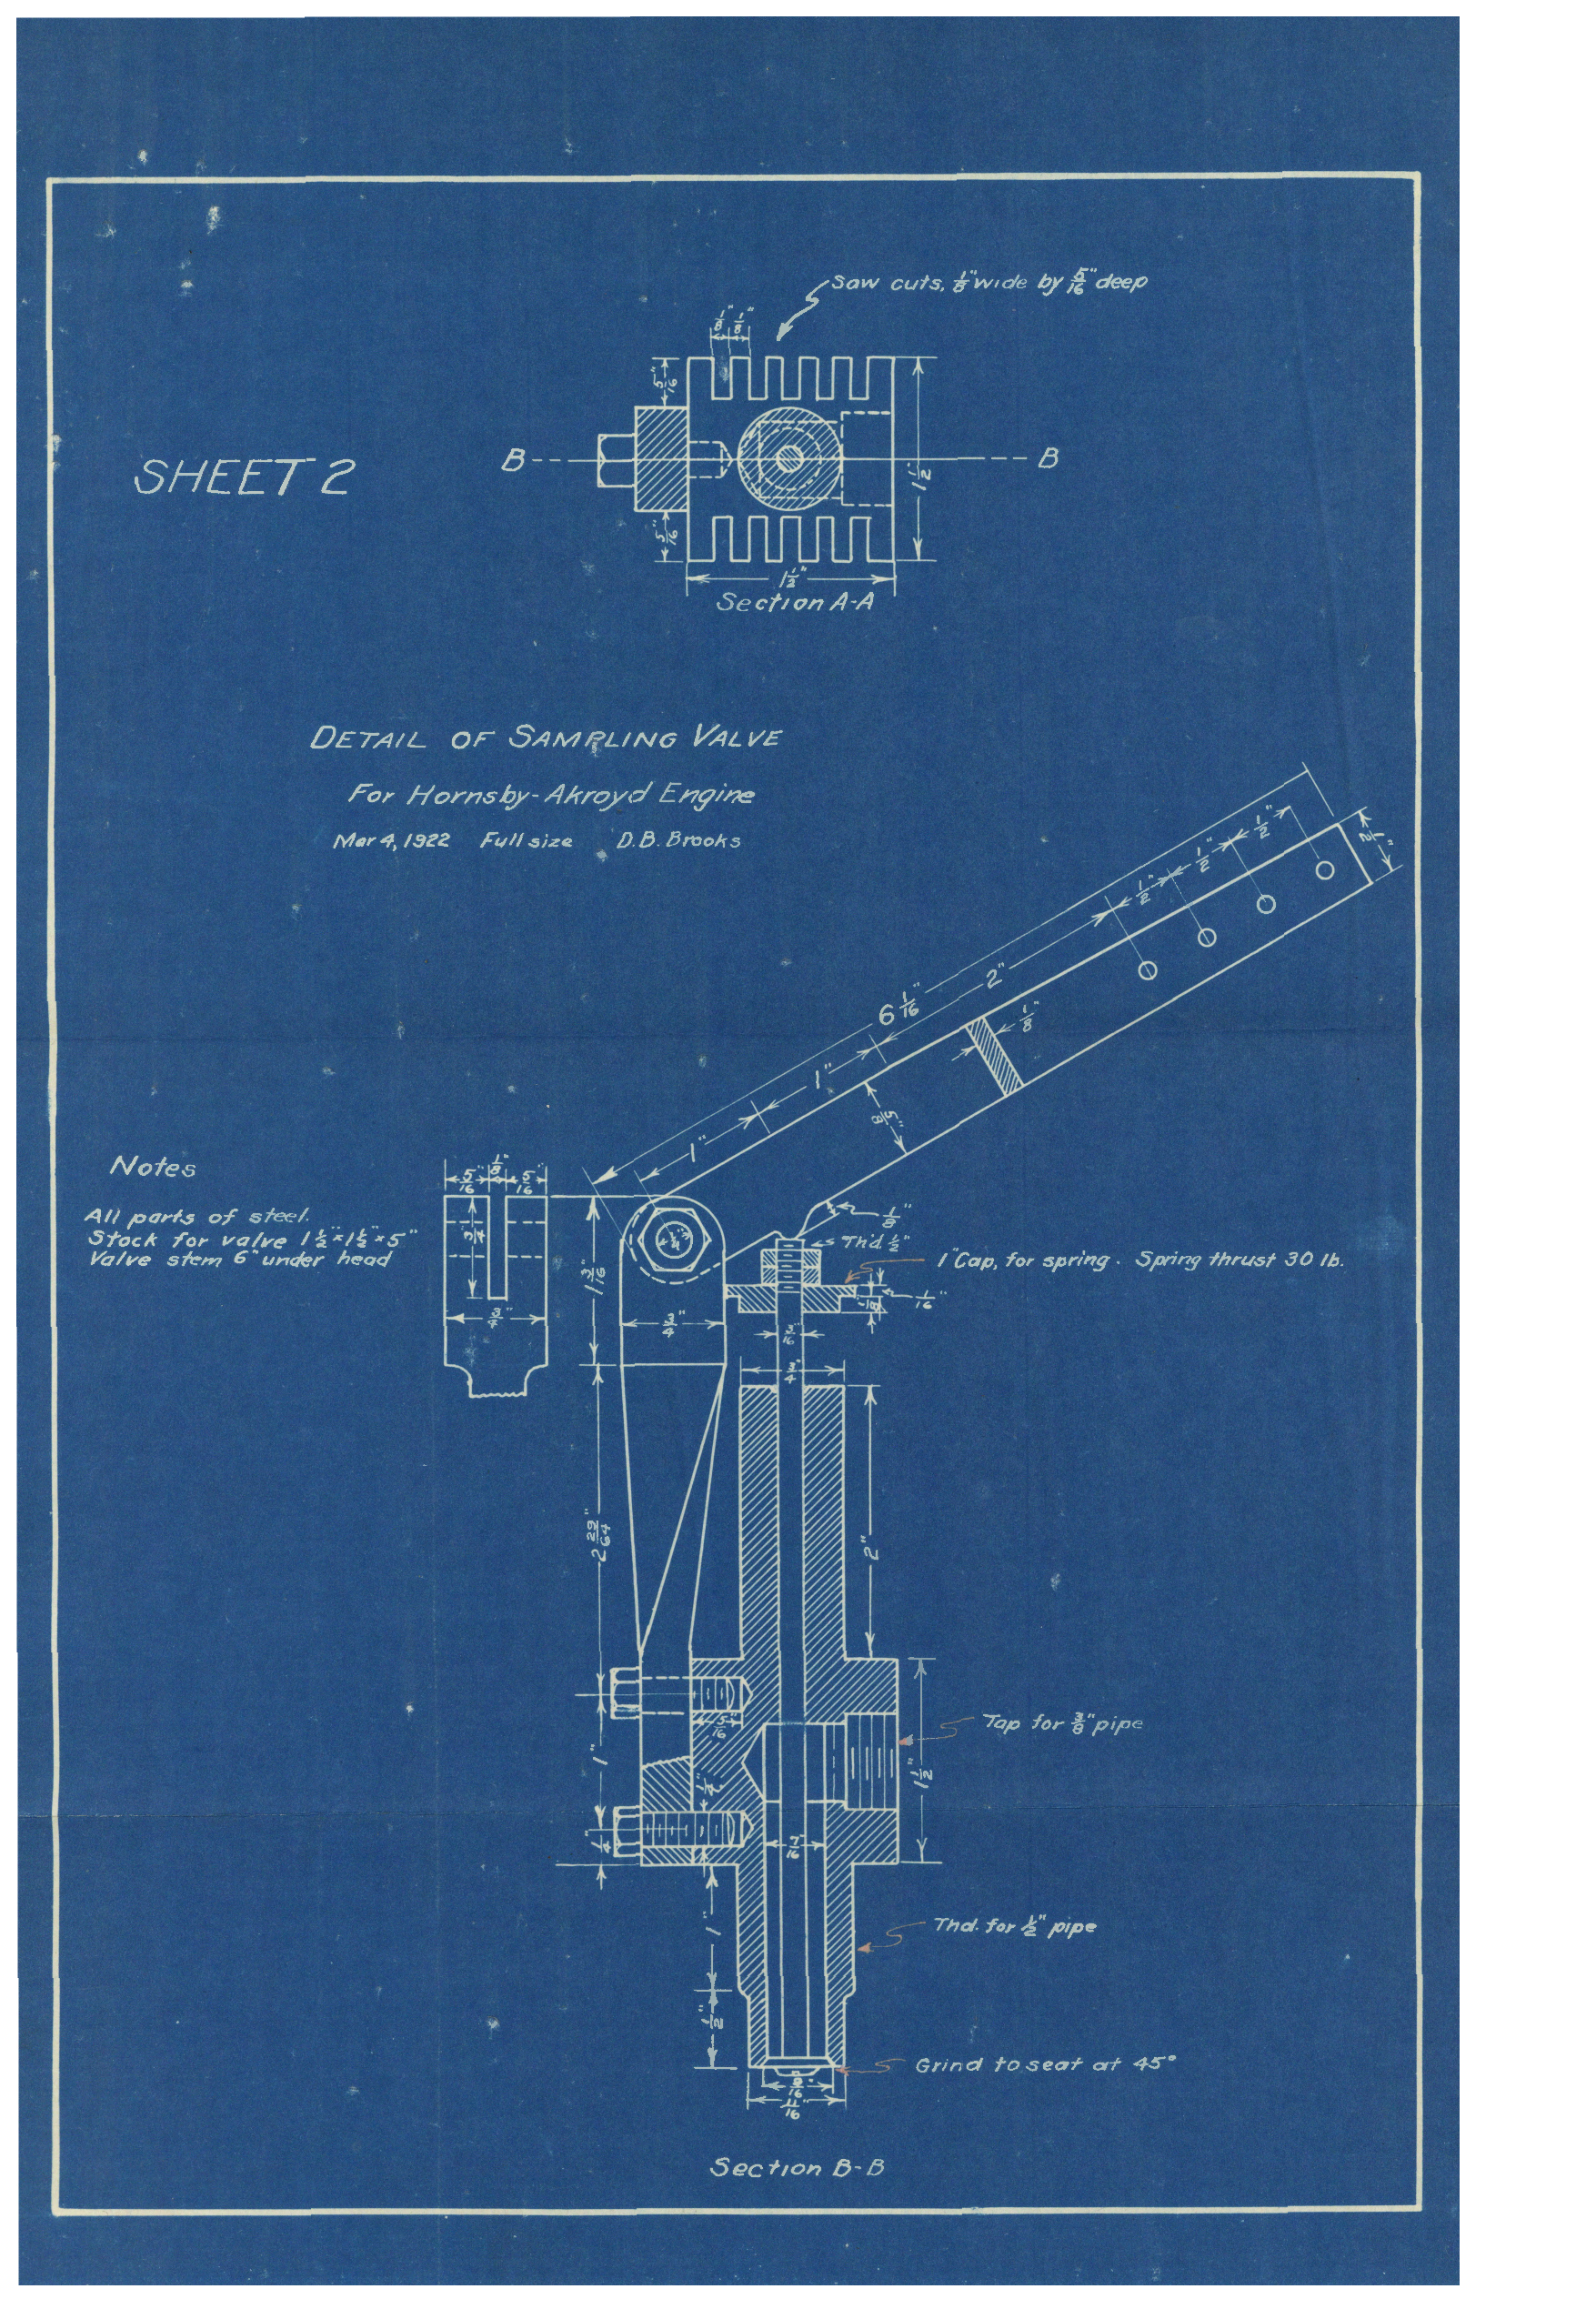
\includegraphics[height=0.95\textheight]{brooks}
                }
                \only<2>{
                    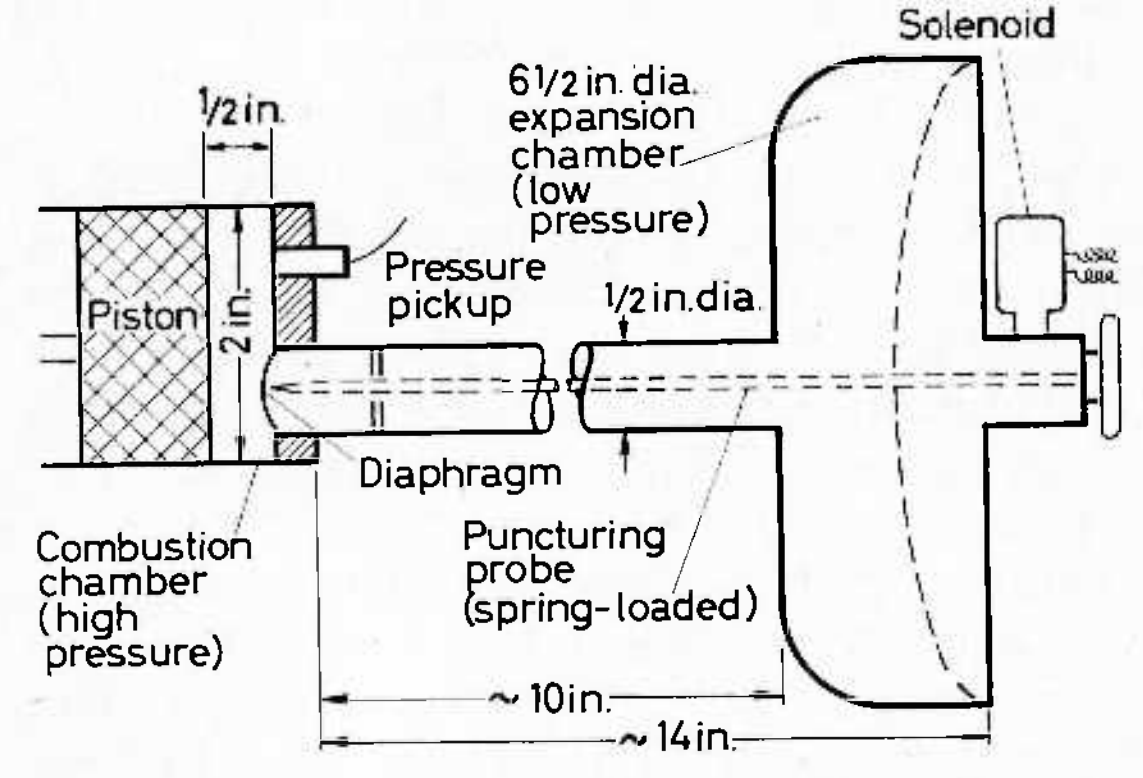
\includegraphics[width=\textwidth]{roblee-sampling}
                }
                \only<3>{
                    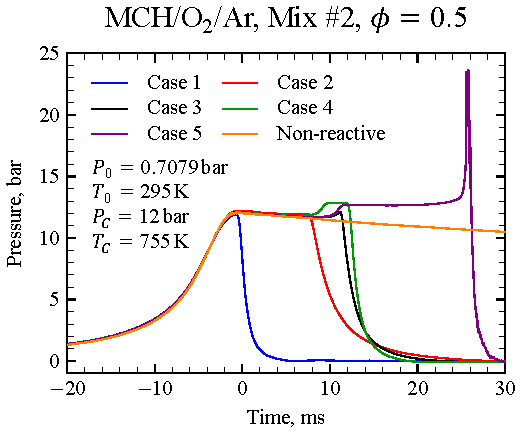
\includegraphics[width=\textwidth]{rsa-pressure}
                }
                \end{minipage}
        \end{columns}
    }
    \begin{center}
        \includegraphics<4>[width=\textwidth,height=0.95\textheight,keepaspectratio]{rcm-schematic}
    \end{center}
\end{frame}

\begin{frame}{Gas Chromatograph/Mass Spectrometer}
    \begin{columns}
        \column{0.4\textwidth}
            \begin{itemize}[<only@+>]
                \item Standard piece of chemistry lab equipment, commercially supplied (Shimadzu GCMS-QP2010S)
                \item Separates, identifies, and quantifies chemical species
            \end{itemize}
        \column{0.6\textwidth}
            \centering
            \includegraphics<1>[width=\textwidth]{gcms-photo}
            \includegraphics<2>[height=0.45\textheight]{gcms-buoh}\par
            \includegraphics<2>[height=0.45\textheight]{mch-tic}
    \end{columns}
\end{frame}

\section{Results}

\begin{frame}{The reactivity of the butanol isomers depends on the pressure}
    \only<1>{
        \begin{columns}
            \column{0.5\textwidth}
                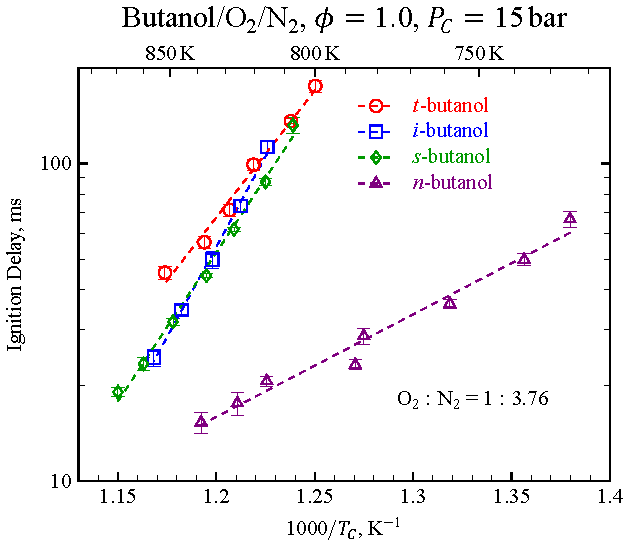
\includegraphics[width=\textwidth]{buoh-15bar}
            \column{0.5\textwidth}
                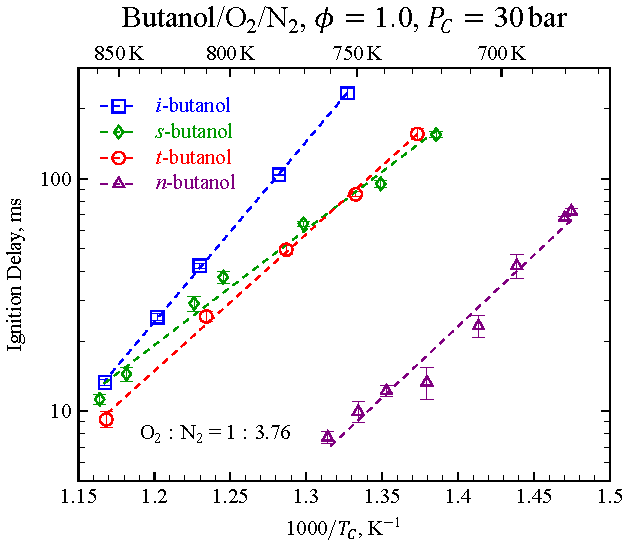
\includegraphics[width=\textwidth]{buoh-30bar}
        \end{columns}
    }
    \begin{center}
        \includegraphics<2>[height=0.85\textheight]{tbuoh-phi20}
    \end{center}
\end{frame}

\begin{frame}{The reactivity trend can be predicted by a detailed understanding of the chemistry}
    \begin{columns}
        \column{0.5\textwidth}
            \includegraphics<1>[width=\textwidth]{buoh-15sim}
            \includegraphics<2>[width=\textwidth]{tbuoh-sims}
        \column{0.5\textwidth}
            \includegraphics<1>[width=\textwidth]{buoh-30sim}
            \includegraphics<2>[width=\textwidth]{tbuoh-20press}
    \end{columns}
\end{frame}

\begin{frame}{My work has lead to substantial improvements in models for hydrocarbons}
    \begin{columns}
        \only<+>{
            \column{0.5\textwidth}
                \centering
                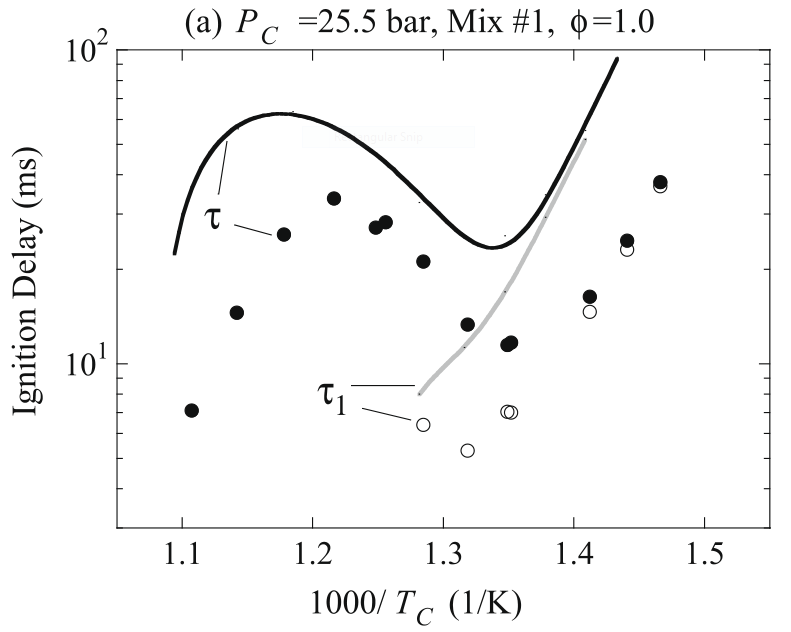
\includegraphics[width=\textwidth]{mittal-mch}\par
                Mittal et al.\ Combust. Flame 2009
            \column{0.5\textwidth}<.>
                \centering
                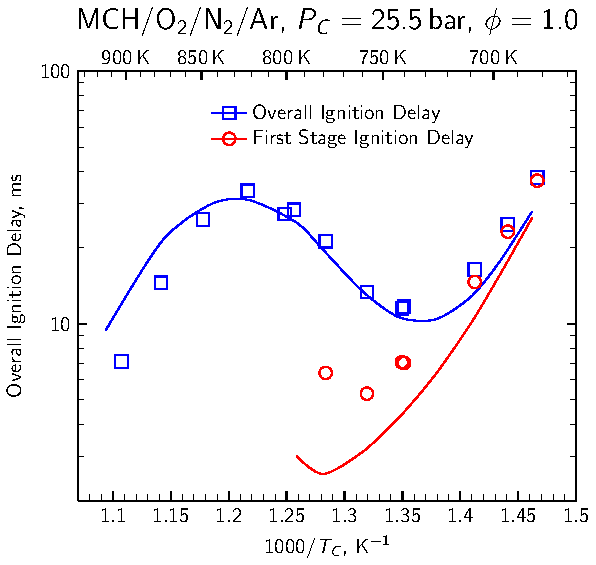
\includegraphics[width=\textwidth]{mch-model-1/mch-model-1}\par
                Weber et al.\ Combust. Flame 2014
        }
    \end{columns}
    \begin{center}
        \includegraphics<+>[height=0.85\textheight]{mch-energy}
    \end{center}
\end{frame}

\begin{frame}{Sampling results}
    \begin{columns}
        \column{0.5\textwidth}
            \centering
            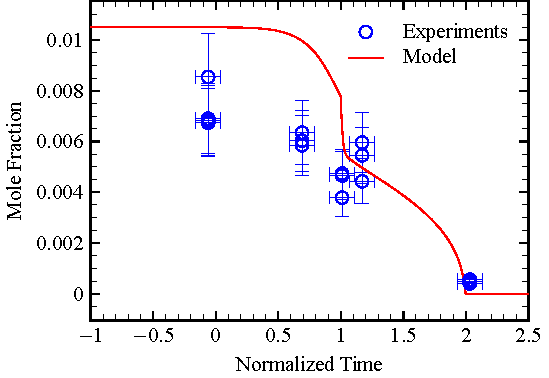
\includegraphics[width=\textwidth]{mch-mole-fracs}
        \column{0.5\textwidth}
            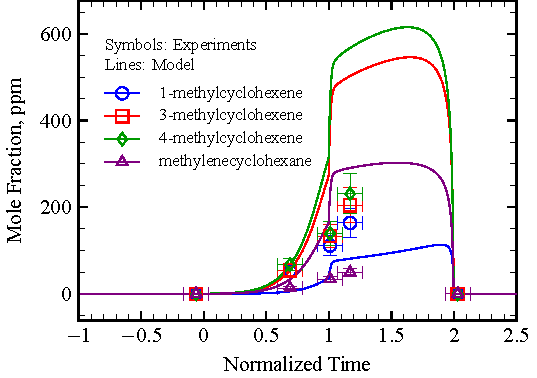
\includegraphics[width=\textwidth]{mchene-mole-fracs}
    \end{columns}
\end{frame}

\begin{frame}{Summary}
    \begin{itemize}
        \item We need a better understanding of the combustion properties of fuels we use now, fuels for the medium-term, and fuels for the long-term especially under engine-relevant conditions
        \item Using this understanding, we need to develop models that can predict the combustion behavior of new fuels in new engines
        \item My dissertation did x y z to advance these causes
    \end{itemize}
\end{frame}

\end{document}
